% =====================================================================
% RESULTS. Finding first, numbers second; every count with its
% denominator; Regime 1 (bf16, sampled) and Regime 2 (fp16, greedy)
% numbers never share a sentence or table. Subsections follow the RQs.
% SOURCES (checked 2026-10-31):
%   Regime 1: Workstream_3/docs/ws3_summary.json and
%     Workstream_3/ws3_results/results/ws3/{mirroring,comparison,factorial,
%     ablation}/**/metrics.json|geometry.json
%   Regime 2: Workstream_3/ws3_results/ada/jobA/analysis/{E-assigned,
%     A-assigned,E-user}/raw.npy + metrics.json, same-pole/metrics.json;
%     judged arms in ada/judged, ada/report, ada/pairwise.
% =====================================================================
\section{Results}
\label{sec:results}

\subsection{The style heads respond to the system prompt, and weakly to the user}
\label{sec:res-heads}

% FLOW R1a: ranks under both sources (finding first) | CHARACTER: the
% style heads | HAND-OFF: ends on "the first token", R1b turns to wording
% SOURCE: ws3_summary.json localization_comparisons (Spearman E/A: resp
% 0.788/0.783, first 0.560/0.616); comparison/*/geometry.json (ranks).
% The fp16 re-run (ada/jobA/analysis) gives the same response-readout ranks.
With the personality in the system prompt, the three style heads are the top three heads of layer 19 for both traits on the response readout (Table~\ref{tab:ranks}). A re-run in half precision, the setting of the removal experiments (Appendix~\ref{app:settings}), reproduces these ranks exactly. With the personality in the user's message, the same three heads still rank among the top four of their layer, and over all 784 heads the assigned and user scores correlate at a Spearman $\rho$ of 0.79 for extraversion and 0.78 for agreeableness. At the first token the picture splits: only head 27 stays near the top for the user contrast, and the correlation falls to 0.56 and 0.62.

\begin{table}[t]
\centering
\small
\begin{tabular}{@{}llcc@{}}
\toprule
Readout & Contrast & Extraversion & Agreeableness \\
\midrule
response & system prompt & 1 / 3 / 2 & 1 / 3 / 2 \\
response & user message & 1 / 2 / 4 & 1 / 2 / 3 \\
response & wording only, high pole & 1 / 3 / 2 & 1 / 2 / 3 \\
response & wording only, low pole & 1 / 2 / 3 & 1 / 2 / 3 \\
first token & system prompt & 2 / 3 / 1 & 2 / 3 / 1 \\
first token & user message & 14 / 10 / 2 & 14 / 13 / 3 \\
\bottomrule
\end{tabular}
\caption{Ranks of heads 2 / 4 / 27 among the 28 heads of layer 19 (1 = largest contribution). Wording-only contrasts pair two system prompts of the same pole and come from the half-precision re-run; the other rows come from the main runs.}
\label{tab:ranks}
\end{table}

% FLOW R1b: the wording-only control and the sizes (Regime 2 numbers only)
% | CHARACTER: the style heads -> head 2 | HAND-OFF: ends on "rewording"
% SOURCE: same-pole/metrics.json (style heads top 3 in all 4 contrasts;
% max |score| on any head 5.96 / 15.69 / 3.59 / 12.16); raw.npy E-assigned
% head 2 = 30.2, heads 4/27 = 8.5/13.6; A-assigned 26.8, 10.7/15.7.
% Ratios: 26.8/12.16 = 2.2 ... 30.2/5.96 = 5.1, 26.8/3.59 = 7.5.
The wording-only control changes how a system prompt is worded while keeping its trait, and it ranks the same three heads first in all four contrasts. The style heads are therefore the heads of layer 19 most sensitive to a change in the system prompt's wording, not only to its personality. Their scores separate them. Head 2 scores 30.2 for the extraversion contrast and 26.8 for agreeableness, while the largest wording-only score on any head ranges from 3.6 to 15.7 across the four contrasts, so head 2 moves 1.9 to 7.5 times more for a change of personality than for a rewording. Heads 4 and 27 score 8.5 to 15.7, comparable to the largest rewording change.

% FLOW R1c: significance is uninformative; then how small and how
% differently oriented the user's signal is | CHARACTER: the test -> the
% user's contrast | HAND-OFF: to behaviour (R2)
% SOURCE: localization fdr counts 669-722 (Regime 1); same-pole fdr
% 688-707 (Regime 2, 999 flips); E-user raw head 2 = 0.72, max any head
% 3.60 at L26 h12; geometry.json cosines and percentiles (Regime 1).
The significance test does not separate heads. In the main runs, 669 to 722 of the 784 heads pass $q < 0.05$ in every localization. In the half-precision re-run, 688 to 707 pass even in the wording-only contrasts, so we interpret ranks and sizes. By size, the user's signal at the style heads is small: in the re-run, the user contrast moves head 2 by 0.7, against 30.2 for the system prompt, and the most user-responsive head in the network is head 12 of layer 26 (score 3.6). In the main runs, the user's signal also points elsewhere. On the response readout, the cosine between the system-prompt and user contrasts inside the style heads is 0.23 for extraversion and 0.38 for agreeableness, near the mean absolute cosine of random three-head groups (0.24 and 0.34). At the first token the cosines are higher, 0.42 and 0.55, at the 85th and 92nd percentiles of random groups.

\subsection{Mirroring is selective}
\label{sec:res-mirroring}

% FLOW R2a: the behavioural table (Regime 1) | CHARACTER: the model's
% replies | HAND-OFF: ends on agreeableness at the ceiling -> pairwise
% SOURCE: ws3/mirroring/metrics.json (E: M 13.05, CI [8.98, 17.05], d_z
% 1.39, p 1.9e-5; poles + 49.00, - 35.95, neutral 33.68; A: M 0.48,
% CI [-0.16, 1.16], d_z 0.31, p 0.097; poles 91.36 / 90.88 / neutral 90.79;
% refusal 0; mean tokens 287-295 of a 300 cap).
Qwen's replies become clearly more extraverted when the user writes in an extraverted style, and barely change when the user is reserved (Table~\ref{tab:mirroring}). Replies to introverted users score 36.0 on the judge's scale, close to the 33.7 of replies to neutral messages, while replies to extraverted users score 49.0. Agreeableness does not move: replies score about 91 whatever the user's style, including for neutral messages, which leaves the absolute scale no room to show a shift. No reply was a refusal, and replies average about 290 of their 300 permitted tokens for every pole.

\begin{table}[t]
\centering
\small
\setlength{\tabcolsep}{4pt}
\begin{tabular}{@{}lccccc@{}}
\toprule
Trait & Neutral & Low & High & $M$ [95\% CI] & $d_z$ \\
\midrule
E & 33.7 & 36.0 & 49.0 & 13.0 [9.0, 17.1] & 1.39 \\
A & 90.8 & 90.9 & 91.4 & 0.5 [$-$0.2, 1.2] & 0.31 \\
\bottomrule
\end{tabular}
\caption{Judged trait of Qwen's replies (0--100) by the style of the user's message, with sampled generation. $M$ is the high-minus-low mirroring effect over 20 requests (Wilcoxon $p = 1.9 \times 10^{-5}$ for E, $0.097$ for A).}
\label{tab:mirroring}
\end{table}

% FLOW R2b: facet and domain splits | CHARACTER: extraversion mirroring |
% HAND-OFF: to pairwise agreeableness
% SOURCE: mirroring/metrics.json per_facet_k (k0 18.46 p 2.1e-4; k1 -1.79
% p 0.67; k2 22.47 p 1.9e-6), per_domain (coding 16.2, explaining 19.4,
% brainstorming 14.0, emotional advice 2.6; n = 5 each).
Extraversion mirroring depends on what the user expresses. Sociable messages raise it to 18.5 points and energetic ones to 22.5, while assertive messages produce no detectable effect ($-1.8$, $p = 0.67$). It also depends on the request: 14.0 to 19.4 points for coding, explanation and brainstorming, against 2.6 for emotional advice. With five requests per domain, these differences are descriptive.

% FLOW R2c: pairwise agreeableness (Regime 2: greedy, 150 tokens) |
% CHARACTER: the pairwise judge | HAND-OFF: to the regression (R3)
% SOURCE: ada/pairwise/A/summary.json (mean_p_high 0.551, CI on p-0.5
% [-0.047, 0.144] -> [0.45, 0.64], Wilcoxon p 0.261, order consistency
% 0.55); ada/pairwise/E/summary.json (0.680, [0.58, 0.78], p 0.0017,
% order consistency 0.65; per facet 0.72 / 0.48 / 0.84).
Pairwise judging of the greedy replies from the removal experiments' reference run agrees with the absolute scores. Shown the replies to a request's extraverted and introverted rewrites, the judge picks the reply to the extraverted user as more extraverted with probability 0.68 (95\% interval [0.58, 0.78], $p = 0.002$), with the facet pattern of the sampled runs: 0.72 for sociable, 0.84 for energetic and 0.48 for assertive messages. Its choice flips with the order of the replies in 35\% of pairs. For agreeableness the probability is 0.55 ([0.45, 0.64], $p = 0.26$), and the choice flips in 45\% of pairs, so the replies to agreeable and disagreeable users are hard to tell apart. We detect no agreeableness mirroring. A pairwise comparison cannot show the asymmetry between the poles, which needs the neutral replies as a reference.

\subsection{The system prompt dominates the style heads}
\label{sec:res-regression}

% FLOW R3: the regression (Regime 1) | CHARACTER: the system prompt -> head
% 2 | HAND-OFF: to zeroing (R4)
% SOURCE: factorial/E-resp and E-first metrics.json. SMH resp R2_A 0.685,
% R2_U 0.006, cos 0.202 [0.162, 0.234]; first R2_A 0.716, R2_U 0.003,
% cos 0.274 [0.223, 0.309]. Groups with head 2: R2_A 0.65-0.72; without:
% 0.10-0.40. User p <= 0.003 in every group. Random cos resp 0.00-0.29,
% first 0.07-0.56. Candidate for the appendix: the full per-group table.
In the crossed set, the system prompt explains far more of the style heads' activity than the user's style does. On the response readout the system-prompt block explains 69\% of the variance and the user block 0.6\% (72\% and 0.3\% at the first token). The user's coefficient is reliably nonzero ($p \le 0.003$ in every head group) and points partly along the system prompt's (cosine 0.20, 95\% interval [0.16, 0.23]), but random triples reach similar or larger cosines, and the style heads have the smallest user share of any group (Appendix~\ref{app:regression}). Head 2 accounts for most of the system prompt's share: every group that contains it explains 65 to 72\% of the variance with the system-prompt block, against 10 to 40\% for groups without it. That block also combines the pole of the system prompt with whether a persona prompt is present at all, two effects we have not separated.

\subsection{Switching the style heads off}
\label{sec:res-zeroing}

% FLOW R4: zeroing (Regime 1) | CHARACTER: zeroing the style heads |
% HAND-OFF: ends on "what they carry", R5 tests the narrower edit
% SOURCE: ablation/*/mirroring/metrics.json (E: 13.69 [10.17, 17.13];
% random [14,17,22] 12.88 [8.38, 17.68]; random [0,1,2] 14.36 [8.98, 19.72];
% A: 0.19 / 0.24 / 0.43). Random [0,1,2] contains head 2.
Switching the style heads off leaves mirroring unchanged: with their output zeroed at every position, the extraversion effect is 13.7 points (95\% interval [10.2, 17.1]), against 13.0 without intervention and 12.9 and 14.4 with two random triples zeroed. One of these triples (heads 0, 1 and 2) contains head 2, which does not change the conclusion because the style heads themselves produced no reduction. Zeroing shows that the style heads are not needed for single-turn mirroring. It cannot show what they carry.

\subsection{Removing the user-style direction}
\label{sec:res-removal}

% FLOW R5a: the removal result, finding first (story doc decision list:
% residual yes; style heads not above the random triple; layer-19 and
% top-10 not above the random direction) | CHARACTER: removing the
% direction | HAND-OFF: to steering (R5b)
% SOURCE: ada/report/metrics.json mirroring_vs_baseline (paired, 5,000
% request resamples): resid -5.46 [-10.12, -0.86] p 0.048, reduction 0.285
% [0.049, 0.512]; smh -1.34 [-4.20, 1.27]; l19 -0.84 [-3.58, 1.93];
% top10 +0.26 [-1.68, 2.31]; rand3 -0.22 [-1.50, 1.18]; randdir +0.40
% [-1.31, 2.07]. Reference M 19.15; coherence 86.8-87.3; refusals 0.
Removing the user-style direction from the residual stream at layer 19 reduces mirroring, and removing it from any group of attention heads does not (Figure~\ref{fig:removal}). Each site uses the user-style direction estimated at that site. In the reference run, with greedy decoding and replies of up to 150 tokens, the mirroring effect is 19.2 points. Removing the direction from the residual stream lowers it by 5.5 points (95\% interval [0.9, 10.1]), a reduction of 29\% (5 to 51\%). It is the only removal whose interval excludes zero, and only just ($p = 0.048$, uncorrected across the eight edits). Removing the direction from the style heads lowers mirroring by 1.3 points ($[-1.3, 4.2]$), and removing it from a random triple lowers it by 0.2 ($[-1.2, 1.5]$). Neither interval excludes zero. Removing it from all 28 heads of layer 19 or from the ten heads most responsive to the user changes mirroring by less than a point, as does a random direction. No edit changes coherence (86.8 to 87.3 against 86.8) or produces a refusal.

\begin{figure*}[t]
\centering
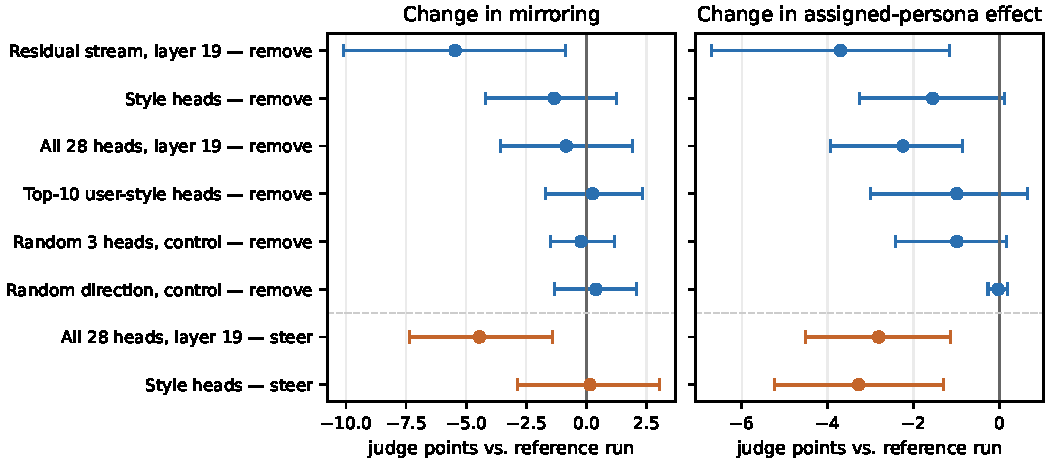
\includegraphics[width=0.85\textwidth]{figures/removal.pdf}
\caption{Paired change from the reference run, with 95\% request-bootstrap intervals, for each edit (greedy decoding). Left: the mirroring effect (19.2 points in the reference run). Right: the effect of an extraverted versus introverted system prompt (65.2 points in the reference run). Blue edits remove the user-style direction. Orange edits reflect it, which is intended to steer towards the opposite style.}
\label{fig:removal}
\end{figure*}

% FLOW R5b: steering | CHARACTER: reflecting the direction | HAND-OFF:
% to preservation (R5c)
% SOURCE: l19_l2 -4.45 [-7.35, -1.40] p 0.012, reduction 0.232 [0.083,
% 0.356]; smh_l2 +0.15 [-2.88, 3.05].
Reflecting the direction separates the layer's heads from the style heads. Reflected across all 28 heads of layer 19, the direction lowers mirroring by 4.4 points ([1.4, 7.3]), a 23\% reduction, while reflected in the style heads alone it leaves mirroring unchanged ($+0.1$, $[-2.9, 3.1]$). The heads of layer 19 together therefore carry a trace of the user's style that affects mirroring when reversed, though not when removed. In the style heads alone we detect none.

% FLOW R5c: persona preservation on the 2x2 | CHARACTER: the assigned
% persona's effect | HAND-OFF: to the RQ answers
% SOURCE: factorial_assigned_vs_baseline: reference 65.22; resid -3.70
% [-6.71, -1.17]; l19_l1 -2.25 [-3.94, -0.86]; l19_l2 -2.81 [-4.52,
% -1.14]; smh_l2 -3.28 [-5.24, -1.29]; smh_l1 -1.55 [-3.26, 0.12];
% randdir -0.03 [-0.27, 0.19]; rand3 -0.99; top10 -0.99. factorial_user:
% reference 2.47; resid -1.83 [-4.10, 0.32]; no arm reliably different.
Every edit along a user-style direction weakens the assigned persona slightly, including edits that leave mirroring unchanged. In the reference run, an extraverted rather than introverted system prompt raises the judged extraversion of the reply by 65.2 points. Removing the residual direction lowers this effect by 3.7 points ([1.2, 6.7]), about 6\%. The other edits lower it by 1.0 to 3.3 points, and the intervals exclude zero for the two layer-wide edits and for reflection at the style heads, which costs 3.3 points ([1.3, 5.2]) without changing mirroring. The random direction leaves the persona's effect unchanged. At the style heads, the user's direction therefore overlaps with what carries the assigned persona, as the positive cosine in Section~\ref{sec:res-regression} suggests. Once a persona is set, the user's own effect is small (2.5 points in the reference run), and no edit changes it reliably.

\subsection{Answers to the research questions}
\label{sec:res-rq}

% FLOW R6: the RQ answers, scoped to single turns and extraversion |
% CHARACTER: each RQ | HAND-OFF: to the Discussion
All answers below come from single exchanges with one model, and the causal tests cover extraversion only.

\textbf{RQ1: Is mirroring driven by a specific, localized computation?} Partly. Removing one direction from the residual stream at layer 19 cuts mirroring by roughly 30\%, with a wide interval. Removing the user's direction from any head group we tested does not, and of the head-level edits only reflecting it across all heads of layer 19 helps. Most of the mirroring survives every edit.

\textbf{RQ2: Do mirroring and the assigned persona share the style heads, or use different pathways?} Largely different pathways. The user's style reaches the style heads only weakly and in a different direction from the system prompt, and editing these heads does not reduce mirroring. Reversing the user's direction there does weaken the assigned persona, so the overlap is not zero.

\textbf{RQ3: Are the two components separable, and can that separation suppress mirroring while preserving the assigned persona?} Partly. Removing the residual-stream direction lowers mirroring by roughly 30\% while the assigned persona keeps about 94\% of its effect, but every edit along a user-style direction costs the persona a little. Suppressing mirroring cleanly would need an edit in the residual stream, or knowing where the user's style is first written.
